\newpage

\anonchapter{Лабораторная работа №5}
\setcounter{chapter}{5}

\begin{center}
Исследование магнетосопротивления полупроводников\\
(4 часа)
\end{center}

\section{Цель работы}
Измерение изменения сопротивления полупроводников в магнитном поле, определение дрейфовой подвижности носителей заряда.

\section{Теоретическая часть}

\subsection{Увеличение электросопротивления полупроводника в магнитном поле}

Эффект магнетосопротивления заключается в изменении электросопротивления обазца при наложении магнитного поля. Причиной возникновения этого эфекта является искривление траектории движения носителей заряда в скрещенных магнитном и электрическом полях.

\begin{figure}[h!]\centering
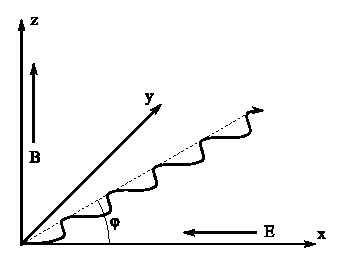
\includegraphics[height=6cm]{pic5_cycloid.eps}
\caption{Траектория электрона в скрещенных электрическом и магнитном полях внутри неограниченного полупроводника}
\label{pic5_cycloid}
\end{figure}

На движущийся заряд в магнитном поле действует сила Лоренца, которая направлена перпендикулярно дрейфовой скорости электронов $\overrightarrow{V}_{d}$ и вектору магнитной индукции $\overrightarrow{B}$. В полупроводнике заряд не может двигаться сколь угодно долго вдоль идеальной траектории, так как испытывает периодические столкновения с дефектами кристаллической решётки. При столкновении теряется энергия и, следовательно, скорость. Таким образом, носители заряда в кристалле двигаются по отрезкам циклоиды (см. рисунок \ref{pic5_cycloid}), при этом среднее направление их движения составляет с направлением поля $\overrightarrow{E}$ некоторый угол $\phi$, называемый углом Холла. Величина угла Холла определяется соотношением между дрейфовой подвижностью носителей $\mu_{d} $ и индукцией магнитного поля:

\begin{equation}
\tg \phi = \mu_{d} B
\end{equation}

Из-за того, что частица движется не по прямой, за время свободного пробега она проходит вдоль поля расстояние меньшее, чем длина свободного пробега $l_{0}$:

\begin{equation}
l_{\text{х}} = l_{0} \cos \phi
\end{equation}

В слабых магнитных полях при малом значении угла Холла

\begin{equation}
l_{\text{х}} = l_{0} \left( 1-\frac{\phi^2}{2} \right) = l_{0} \left( 1-\frac{\mu_{d}^2 B^2}{2} \right)
\end{equation}

Уменьшение пути $l_{\text{х}}$ эквивалентно уменьшению проводимости проводника:

\begin{equation}
\frac{\Delta \rho}{\rho_{0}} = \frac{\rho_{B} - \rho_{0}}{\rho_{0}} = \frac{\sigma_{0} - \sigma_{B}}{\sigma_{B}} = \frac{\l_{0} - \l_{\text{х}}}{\l_{\text{х}}} \approx \frac{\mu_{d}^2 B^2}{2}
\end{equation}

Изменение электросопротивления полупроводника пропорционально квадрату индукции магнитного поля, при этом коэффициент пропорциональности определяется величиной дрейфовой подвижности.

\subsection{Величина магнетосопротивления в ограниченном полупроводнике}

\begin{figure}[h!]\centering
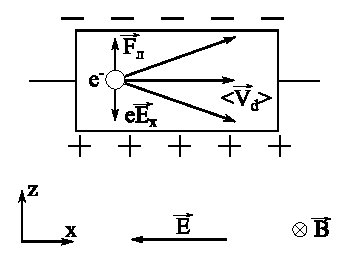
\includegraphics[height=6cm]{pic5_strip.eps}
\caption{Направления движения электронов в ограниченном образце в скрещенных электрическом и магнитном полях}
\label{pic5_strip}
\end{figure}

Рассмотрим полупроводник в виде длинного однородного стержня (рис. \ref{pic5_strip}). Под действием электрического поля $\overrightarrow{E}$ электроны движутся вдоль оси $x$. Со стороны магнитного поля $\overrightarrow{B} \perp \overrightarrow{E}$ на электроны действует сила Лоренца, направленная вдоль оси $z$. Двигаясь под действием силы Лоренца электроны скапливаются на одной из граней, заряжая её отрицательно. На противоположной грани образцется положительный заряд нескомпенсированных ионов примеси. В результате возникает поперечная ЭДС Холла, препятствующая дальнейшему разделению зарядов. Накопление зарядов будет продолжаться до тех пор, пока поле Холла не скомпенсирует отклоняющее действие магнитного поля:

\begin{equation}
e \overrightarrow{E} = -e \left[ \overrightarrow{V}_{d} \times \overrightarrow{B} \right]
\end{equation}

Если бы все электроны в кристалле имели одинаковые скорости, то они двигались бы прямолинейно вдоль оси Ox, так как кулоновская сила создаваемая полем Холла уравновешивается силой Лоренца. Однако в полупроводнике всегда имеет место некоторое распределение электронов по скоростям, обусловленное вероятностным характером рассеяния носителей. Из-за этого электроны, обладающие скоростью ниже средней будут отклоняться к одной грани образца под действием нескомпенсированного поля Холла, а обладающие более высокой скоростью - к другой, под действием нескомпенсированной силы Лоренца. При этом поток электронов в направлении приложенного поля уменьшается, что приводит к уменьшению электропроводности. За счёт того, что продольная скорость уменьшается только для электронов со скоростями, далёкими от средней, увеличение электросопротивления будет менее заментым, нежели в неограниченном образце. В вырожденных полупроводниках и металлах в проводимости участвуют прежде всего электроны, находящиеся вблизи уровня Ферми и обладающие поэтому практически одинаковыми скоростями, поэтому эффект Холла в них будет заметен гораздо меньше, чем в невырожденных полупроводниках.

Более строгий вывод эффекта магнетосопротивления может быть проведён на основе решения кинетического уравнения Больцмана. Решением являются выражения для электропроводности в присутствии магнитного поля

\begin{equation}
\sigma_{B} = e n \left< \frac{\mu}{1 + \mu^2 B^2} \right>
\end{equation}

В области слабых магнитных полей ($\mu B \ll 1$) 

\begin{equation}
\frac{\Delta \rho}{\rho_{0}} = \frac{<\mu^3>}{<\mu>} B^2 = \frac{<\mu^3>}{<\mu>^3}\mu^{2}_{d} B^2 = \frac{<\tau^3>}{<\tau>^3}\mu^{2}_{d} B^2 = C \mu^{2}_{d} B^2
\end{equation}

Величина $C$ характеризует разброс носителей по скоростям и определяется доминирующим механизмом рассеяния.

В сильном магнитном поле ($\mu B \gg 1$) 

\begin{equation}
\frac{\Delta \rho}{\rho_{0}} = \frac{<\mu>}{<\mu^{-1}>} B^2 = \frac{1}{<\mu><\mu^{-1}>} \mu_{d}^2 B^2 = \frac{1}{<\tau><\tau^{-1}>} \mu_{d}^2 B^2
\end{equation}

Для ограниченного полупроводника с одним типом носителей, имеющего форму бесконечно длинного стержня, в области слабых магнитных полей ($\mu B \ll 1$) можно считать, что

\begin{equation}
\frac{\Delta \rho}{\rho_{0}} = [C - A^2] \mu^{2}_{d} B^2
\end{equation}
где $C = \frac{\left< \tau^3 \right>}{\left< \tau \right>^3}$, $A = \frac{\left< \tau^2 \right>}{\left< \tau \right>^2}$ - холл-фактор.

Величина $C$ определяет магнетосопротивление, обусловленное искривлением траектории носителей заряда в магнитном поле. Величина $A^2$ - компенсирующее действие поля Холла. В таблице \ref{table5_koef} приведены значения этих величин для некоторых механизмов рассеяния, считая, что зависимость времени релаксации от энергии степенная: $\tau(E) \approx E^p$

\begin{table}[h!]
\caption{Величины коэффициентов в выражении для магнетосопротивления}
\begin{center}
\begin{tabular}{c|c|c|c|c}
p & $-1/2$ & $0$ & $1/2$ & $3/2$ \\
\hline
C & $\frac{9 \pi}{16} \approx 1.77$ & 1 & $\frac{27 \pi}{64} \approx 1.33$ & $\frac{15 \pi}{8} \approx 5.90$ \\
$A^2$ & $\frac{3 \pi}{8} \approx 1.18$ & 1 & $\frac{45 \pi}{128} \approx 1.10$ & $\frac{315 \pi}{512} \approx 1.93$ \\
$C-A^2$ & 0.38 & 0 & 0.11 & 2.15 \\
\hline
\end{tabular}
\end{center}
\label{table5_koef}
\end{table}

На величину эффекта магнетосопротивления существенное влияние оказывает форма образца. Окооло токовых онтактов линии тока в образце изгибаются, так как металлизация контакта закорачивает поле Холла. При уменьшении отношения длины образца к его ширине вклад приконтактных областей в относительное изменение сопротивления образца возрастает.

\subsection{Диск Корбино}
Удобной моделью неограниченного образца является диск Корбино - образец, выполненный в форме диска с отверстием в центре (рис. \ref{pic5_korbino}). Токовые контакты в таком образце расположены в центральном отверстии и по периферии диска, а магнитное поле направлено перпендикулярно плоскости диска. Линии тока наравлены от цента к краям по радиусу. Под действием магнитного поля линии тока в образце искривляются, но поперечное к электрическому поле Холла не возникает, так как не происходит разделения зарядов в образце.

\begin{figure}[h!]\centering
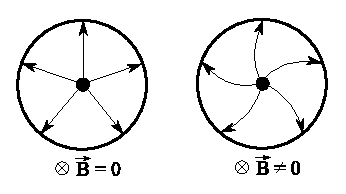
\includegraphics[height=6cm]{pic5_korbino.eps}
\caption{Линии тока в образце, выполненном в виде диска Корбино}
\label{pic5_korbino}
\end{figure}

Если в полупроводнике присутствуют несколько типов носителей заряда, то рассмотрение эффекта магнетосопротивления усложняется. Для ограниченного полупроводника со смешанной проводимостью в слабом магнитном поле $(\mu B \ll 1)$

\begin{equation}
\frac{\Delta \rho}{\rho_{0}} = C \frac{1+ x b^3}{1 + x b} \mu_{p}^{2} B^{2} - A^{2} \frac{(1 - x b^2)^2}{(1 + x b)^2} \mu_{p}^{2} B^{2}
\end{equation}
где $x = \frac{n}{p}$, $b = \frac{\mu_{n}}{\mu_{p}}$.

При переходе к собственной проводимости относительное изменение сопротивления может возрастать, так как уменьшается компенсирующее действие поля Холла. В собственном полупроводнике с $\mu_{n} = \mu_{p}$ поле Холла отсутствовало бы, и второе слагаемое оказалось бы равно нулю.

\section{Методика измерений и описание установки}

Схема установки для измерения магнетосопротивления приведена на рисунке \ref{pic5_scheme}.

\begin{figure}[h!]\centering
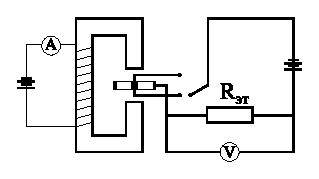
\includegraphics[height=6cm]{pic5_scheme.eps}
\caption{Блок-схема установки для измерения электросопротивления}
\label{pic5_scheme}
\end{figure}

В зазор между полюсами электромагнита устанавливается полупроводник в форме диска Корбино. Величина магнитного поля задаётся высокоточным выпрямителем и рассчитывается по градуировочной кривой. Определение сопротивления образца определяется по сравнению падения напряжения на образце $(U_{\text{обр}})$ и на эталонном сопротивлении $(U_{\text{э}})$. Величина эталонного сопротивления составляет 10 Ом. Переключение между образцом и эталоном производится при помощи тумблера.
Величина $(U_{\text{обр}})$ определяется при помощи цифрового вольтметра. Для исключения влияния термоЭДС напряжение измеряется при двух различных направлениях тока. Так как при перемене направления тока через образец $(U_{\text{обр}})$ меняет свою полярность, а полярность $(U_{\text{ТЭДС}})$ зависит только от градиента температур, то можно считать, что

\begin{equation}
\begin{split}
U_{1} &= U_{\text{обр}} + U_{\text{ТЭДС}} \\
U_{2} &= - U_{\text{обр}} + U_{\text{ТЭДС}} \\
U_{\text{обр}} &= \frac{U_{1} - U_{2}}{2}
\end {split}
\end{equation}

Сопротивление образца можно рассчитать по формуле

\begin{equation}
R = R_{\text{эт}} \frac{U_{\text{обр}}}{U_{\text{эт}}}
\end{equation}

Зная, как меняется величина электросопротивления, можно определить величину дрейфовой подвижности $\mu_{d}$. Для образца с одним типом носителей, имеющего форму диска Корбино

\begin{equation}
\frac{\Delta R}{R_{0}} = \frac{\Delta \rho}{\rho_{0}} = C \mu_{d}^2 B^2 \rightarrow
\left( \frac{\Delta R}{R_{0}} \right)^{1/2} = C^{1/2} \mu_{d} B
\label{eq5_muB}
\end{equation}

\section{Порядок проведения работы и указания по технике безопасности}

\begin{enumerate}
\item Установить образец между полюсами электромагнита.
\item Задать ток через схему, регулируя напряжение источника и фиксируя падение напряжения на эталонном сопротивлении.
\item Измерить падение напряжения на эталоне $U_{\text{эт}}$
\item Измерить падение напряжения на образце $U_{\text{обр}}$ меняя ток в электромагните от 0 до 2 А с шагом 200 мА.
\item Результаты занести в таблицу \ref{5_table}
\end{enumerate}

В ходе работы соблюдать стандартную технику безопасности при обслуживании высокоточных (до 3 А) источников, а также высоких (до 0,5 Тл) магнитных полей.

\begin{table}[h!]
\caption{Измерение магнетосопротивления}
\begin{center}
\begin{tabular}{c|c|c|c|c|c|c|c|c}
№ & $I_{\text{обр}}$ & $I_{\text{магн}}$ & B & $U_{\text{эт}}$ & $U_{\text{обр}}^{+}$ & $U_{\text{обр}}^{-}$ & $R_{\text{обр}}$ & $\left( \frac{\Delta R}{R_{0}} \right)^{1/2}$ \\
\hline
& мА & А & Тл & мВ & мВ & мВ & Ом & \\
\hline
\end{tabular}
\end{center}
\label{5_table}
\end{table}

\section{Обработка результатов эксперимента}
\begin{enumerate}
\item Для нахождения величины дрейфовой подвижности строится зависимость $\left( \frac{\Delta R}{R_{0}} \right)^{1/2} = f(B)$. Она должна иметь вид прямой линии.
\item Из тангенса угла наклона прямой можно в соответствии с формулой (\ref{eq5_muB}) найти дрейфовую подвижность материала.
\end{enumerate}

\section{Контрольные вопросы}
\begin{enumerate}
\item Движение новителей заряда в скрещенных электрическом и магнитном полях.
\item Подвижность носителей заряда. Холловская и дрейфовая подвижности.
\item Эффект магнетосопротивления в неограниченном полупроводнике.
\item Эффект магнетосопротивления в ограниченном полупроводнике.
\item Влияние поля Холла на эффект магнетосопротивления.
\item Зависимость магнетосопротивления от величины магнитной индукции.
\item Влияние формы образца на величину эффекта магнетосопротивления.
\item Эффект магнетосопротивления в полупроводнике с несколькими типами носителей заряда.
\item Относительное изменение удельного электросопротивления неограниченного полупроводника в слабом магнитном поле.
\item Определение подвижности из измерений эффекта магнетосопротивления.
\item Ошибки, ограничивающие точность определения дрейфовой подвижности.
\end{enumerate}

\section{Литература}
\begin{enumerate}
\item П.С. Киреев. Физика полупроводников. СПб.: Лань, 2011 г.
\item В.В. Батавин, Ю.А. Концевой, Ю.В. Федорович. Измерение параметров полупроводниковых материалов и структур. М.: Радио и связь, 1985 г.
\end{enumerate}